% [原文 p.51]
\chapter{Jones--Witten 理论}

本章考察定义在共形块丛上的 KZ 联络的和乐结构。作为这一和乐，辫群的表示会出现；利用它，可以自然地得到链环的拓扑不变量------Jones 多项式。三维流形的 Witten 不变量，本来是以 Chern--Simons 泛函的配分函数的形式提出的；本书则从共形场论的和乐这一立场来构造 Witten 不变量。进一步，从这样的观点出发，将说明共形场论给出 Atiyah 意义下的拓扑场论的例子。此外还将涉及 Chern--Simons 理论与曲面上联络空间几何的关系，说明由共形场论给出的构造与 Chern--Simons 理论的途径之间的关联。

\section{KZ 方程与辫群的表示}

\takeaway{KZ 方程是以 $\kappa$ 为参数、定义在构形空间 $\Conf_n(\C)$ 上的一族全微分方程；方程 (2.9) 表明联络形式平方为零，由此得到的平坦联络，其解沿道路的解析延拓给出纯辫群 $P_n$ 与辫群 $B_n$ 的线性表示，即 KZ 方程的单值表示。}

对复向量空间 $\C^n$，把由 $z_i=z_j$ 定义的超平面记作 $H_{ij}$。复平面 $\C$ 上 $n$ 个互异点的构形空间 $\Conf_n(\C)$，按定义表为
\[
  \Conf_n(\C)=\C^n\setminus\bigcup_{i<j}H_{ij}.
\]
$\Conf_n(\C)$ 的基本群称为纯辫群（pure braid group），记作 $P_n$。又，$n$ 次对称群 $S_n$ 通过坐标的置换作用在 $\Conf_n(\C)$ 上，
% [原文 p.52]
由此作用得到的商空间 $Y_n=\Conf_n(\C)/S_n$ 的基本群称为辫群（braid group），记作 $B_n$。存在自然的满射 $p:B_n\to S_n$，其核 $\Ker p$ 即纯辫群 $P_n$。辫群 $B_n$ 的元素，如图 2.1 所示，可以表示为 $n$ 条互不相交的绳子的同痕类。已知 $B_n$ 由图 2.1 所示的生成元 $\sigma_i$（$i=1,\dots,n-1$）以及它们之间的关系式
\begin{align}
  \sigma_i\sigma_{i+1}\sigma_i&=\sigma_{i+1}\sigma_i\sigma_{i+1}, & i&=1,\cdots,n-2, \tag{2.1}\\
  \sigma_i\sigma_j&=\sigma_j\sigma_i, & |i-j|&>1 \tag{2.2}
\end{align}
给出。

% [Tutor Note: 式 (2.1)、(2.2) 即 Artin 辫群的标准表示：相邻生成元之间是辫关系，不相邻生成元之间交换。第二式的条件 $|i-j|>1$ 表达的是“不相邻”，不是 $i\ne j$，两者常被混淆。]

\begin{figure}[htbp]
  \centering
  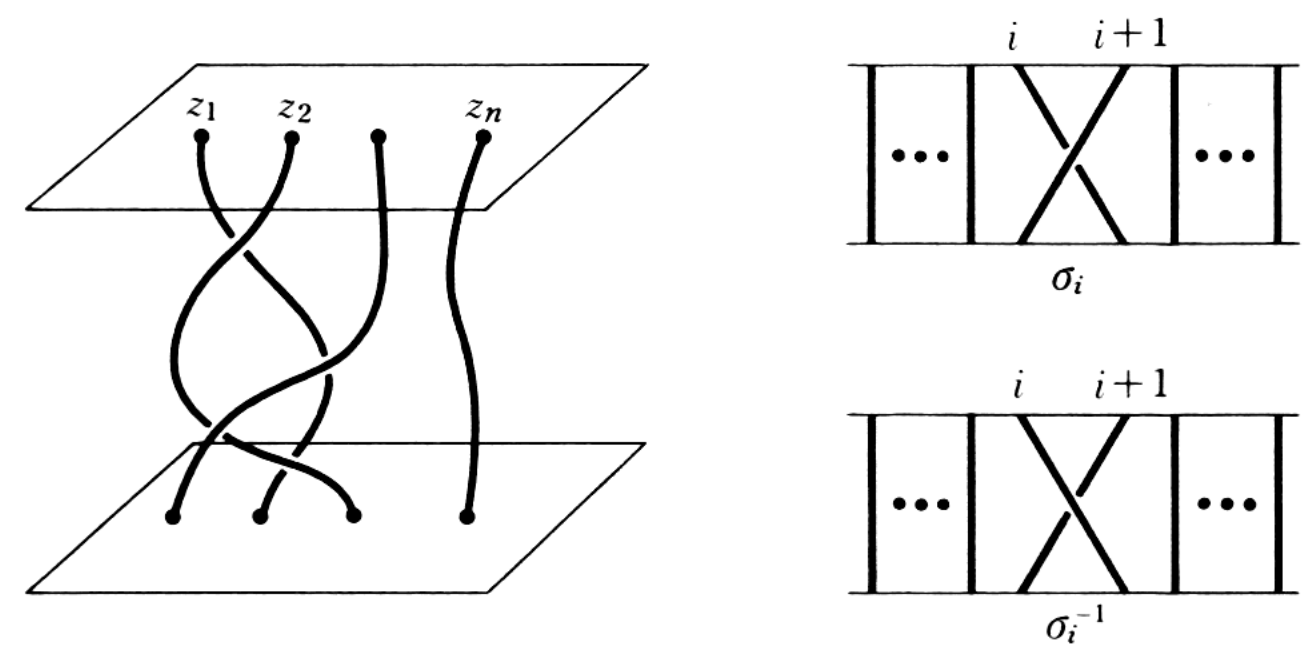
\includegraphics[width=0.86\textwidth]{figures/fig2.1.png}
  \figtitle{2.1}{辫群及其生成元（原书 p.52）}
\end{figure}

在构形空间 $\Conf_n(\C)$ 上，考虑对数微分形式
\[
\begin{aligned}
  \omega_{ij}&=\rd\log(z_i-z_j)\\
  &=\frac{\rd z_i-\rd z_j}{z_i-z_j},\qquad i\ne j.
\end{aligned}
\]
它们满足二次关系式
\begin{equation}
  \omega_{ij}\wedge\omega_{jk}+\omega_{jk}\wedge\omega_{ki}+\omega_{ki}\wedge\omega_{ij}=0,
  \qquad i<j<k. \tag{2.3}
\end{equation}

% [Tutor Note: 记号写作 $\rd\log(z_i-z_j)$，但 $\log$ 有分支，它没有单值的原函数；作为一次微分形式，它在 $\Conf_n(\C)$ 上整体定义且闭。又 $\omega_{ji}=\omega_{ij}$，故 (2.3) 三项是同一形式按 $i<j<k$ 循环取值的和。]

第 1.5 节曾把 KZ 方程作为共形块丛上自然出现的平坦联络引入；这里对一般的有限维复单 Lie 代数重新表述 KZ 方程。固定有限维复单 Lie 代数 $\fg$ 及其一族表示 $\rho_j:\fg\to$
% [原文 p.53]
$\End(V_j)$，$1\le j\le n$。取 $\fg$ 关于 Cartan--Killing 型的标准正交基 $\{I_\mu\}$。令 $\Omega=\sum_\mu I_\mu\otimes I_\mu$；把 $\Omega$ 作用在 $V_1\otimes V_2\otimes\cdots\otimes V_n$ 的第 $i$ 个与第 $j$ 个张量因子上，所得到的线性变换记作 $\Omega_{ij}$（$i\ne j$）。也就是说，令
\begin{equation}
  \Omega_{ij}=\sum_\mu 1\otimes\cdots\otimes\rho_i(I_\mu)\otimes\cdots\otimes\rho_j(I_\mu)\otimes\cdots\otimes 1. \tag{2.4}
\end{equation}
所谓 KZ 方程，是关于 $\Conf_n(\C)$ 上取值于 $V_1\otimes V_2\otimes\cdots\otimes V_n$ 的函数 $\Phi(z_1,\dots,z_n)$ 的微分方程
\begin{equation}
  \frac{\partial\Phi}{\partial z_i}
  =\frac{1}{\kappa}\sum_{j,\,j\ne i}\frac{\Omega_{ij}\Phi}{z_i-z_j}. \tag{2.5}
\end{equation}
其中 $\kappa$ 是复参数。若令
\[
  \omega=\frac{1}{\kappa}\sum_{1\le i<j\le n}\Omega_{ij}\omega_{ij},
\]
则 KZ 方程也可以写成全微分方程
\begin{equation}
  \rd\Phi=\omega\Phi \tag{2.6}
\end{equation}
的形式。

% [Tutor Note: 参数 $\kappa$ 与共形场论的 level $k$ 由 $\kappa=k+h^\vee$ 相联系（$h^\vee$ 为对偶 Coxeter 数）；本书后面取 $\fg=\fsl_2(\C)$ 时 $h^\vee=2$，故 $\kappa=k+2$。与文献对比时这一步平移最易出错。]

关于 $\Omega_{ij}$，成立下述引理。

\begin{lemma*}{2.1}
  $\Omega_{ij}$（$1\le i,j\le n$）满足关系式
  \begin{align}
    [\Omega_{ij}+\Omega_{jk},\Omega_{ik}]&=0 &&(i,j,k\ \text{互不相同}), \tag{2.7}\\
    [\Omega_{ij},\Omega_{kl}]&=0 &&(i,j,k,l\ \text{互不相同}). \tag{2.8}
  \end{align}
\end{lemma*}

% [Tutor Note: 这里 $\{I_\mu\}$ 是 $\fg$ 关于 Cartan--Killing 型的标准正交基，$\Omega=\sum_\mu I_\mu\otimes I_\mu$ 与基的选取无关，是 Casimir 元在张量积上的作用；$\Omega_{ij}$ 只在前述两个因子上非平凡，其余因子取恒等映射。]

\begin{proof}
  式 (2.8) 是显然的。(2.7) 的证明如下：$C=\sum_\mu I_\mu\cdot I_\mu$ 是所谓 Casimir 元，属于 Lie 代数泛包络代数 $U(\fg)$ 的中心；利用余积 $\Delta:U(\fg)\to U(\fg)\otimes U(\fg)$，$\Omega$ 可表为
  \[
    \Omega=\frac{1}{2}\left(\Delta C-C\otimes 1-1\otimes C\right),
  \]
  由此即得 (2.7)。
\end{proof}

与式 (2.3) 合并，得到
% [原文 p.54]
\begin{equation}
  \omega\wedge\omega=0. \tag{2.9}
\end{equation}
$\omega$ 满足 $\rd\omega=0$，故
\[
  \rd\omega+\omega\wedge\omega=0.
\]
因此，以 $\Conf_n(\C)$ 为底空间、以 $V_1\otimes V_2\otimes\cdots\otimes V_n$ 为纤维的平凡向量丛，其联络若由 $\nabla=\rd-\omega$ 定出，则该联络的曲率为 $0$。也就是说，$\omega$ 给出平坦联络。

% [Tutor Note: 平坦性 = 曲率为零，即 $\rd\omega+\omega\wedge\omega=0$；此处 $\rd\omega=0$ 与 (2.9) 各贡献一项。注意 $\omega$ 是矩阵值一次形式，$\rd\omega$ 与 $\omega\wedge\omega$ 的次序不可随意交换。]

作为联络 $\nabla$ 的和乐，得到以 $\kappa$ 为参数的纯辫群的线性表示
\[
  \theta:P_n\longrightarrow\End(V_1\otimes\cdots\otimes V_n).
\]
具体地说，$\theta$ 这样确定。首先，对于以 $x_0$ 为基点的 $\Conf_n(\C)$ 的环路 $\gamma$，在基点 $x_0$ 附近取全微分方程 (2.6) 的一组线性无关解 $(\Phi_1,\dots,\Phi_m)$，其中 $m=\dim V_1\times\cdots\times\dim V_n$；沿 $\gamma$ 解析延拓之后，在 $x_0$ 附近所得的解表为
\[
  (\Phi_1,\dots,\Phi_m)\theta(\gamma).
\]
由于 $\nabla$ 是平坦联络，$\theta(\gamma)$ 只由 $\gamma$ 的同伦类决定。这样，从任意复单 Lie 代数 $\fg$ 及其表示出发，就得到了作为 KZ 联络的和乐的纯辫群线性表示。称之为 KZ 方程的单值表示（monodromy representation）。又，当 $V_1=\cdots=V_n=V$ 时，用对称群 $S_n$ 的对角作用去除平凡向量丛 $E=\Conf_n(\C)\times V^{\otimes n}$，便可在 $Y_n$ 上构成以 $V^{\otimes n}$ 为纤维的向量丛 $F$。这里，对称群在 $V^{\otimes n}$ 上的作用由张量积各因子的置换定义。联络 $\nabla$ 在该对称群作用下不变，故在向量丛 $F$ 上定出联络；其和乐给出辫群的线性表示
\[
  \theta:B_n\longrightarrow\End(V^{\otimes n}).
\]

% [Tutor Note: 解按列排成 $m\times m$ 矩阵 $(\Phi_1,\dots,\Phi_m)$，单值矩阵右乘；故 (2.16) 中 $F$ 的左乘、右乘位置要与 $\Phi_1,\Phi_2$ 的排法对照，不能只记式子。]

下面回到共形块的情形，考察 KZ 方程单值表示的结构。处理第 1.4 节所定义的、对应于 $\fg=\fsl_2(\C)$ 的 level $k$ 的共形块空间。首先，在 $\CP^1$ 上取互异的 3 点 $p_1,p_2,p_3$ 以及 $p_4=\infty$，对它们分别赋予 level $k$ 的最高权 $\lambda_1,\lambda_2,\lambda_3,\lambda_4^*$，考察共形块的空间 $\cH(\bm{p},\bm{\lambda})$。这个共形块的空间可以嵌入不变张量的空间
% [原文 p.55]
\begin{equation}
  V^{\lambda_4}_{\lambda_1\lambda_2\lambda_3}
  =\Hom_{\fg}\left(V_{\lambda_1}\otimes V_{\lambda_2}\otimes V_{\lambda_3},\,V_{\lambda_4}\right). \tag{2.10}
\end{equation}
在 $\Conf_3(\C)$ 上考虑以共形块的空间 $\cH(\bm{p},\bm{\lambda})$ 为纤维的共形块丛，把各纤维嵌入上述不变张量空间 (2.10)；此时式 (2.5) 中取 $n=3$、$\kappa=k+2$ 所得者，给出该向量丛的平坦联络 $\nabla$。这里 $z_1,z_2,z_3$ 分别表示 $p_1,p_2,p_3$ 的坐标。KZ 方程在平移下不变，故可令 $z_1=0$。作坐标变换 $z_2=u_1u_2$、$z_3=u_2$，把三重交点 $z_1=z_2=z_3$ 爆破，则 $\omega$ 在 $u_1=u_2=0$ 附近表为
\begin{equation}
  \omega=\frac{1}{\kappa}\left(
  \frac{\Omega_{12}\,\rd u_1}{u_1}
  +\frac{(\Omega_{12}+\Omega_{13}+\Omega_{23})\,\rd u_2}{u_2}
  +\omega_1\right) \tag{2.11}
\end{equation}
的形状。其中 $\omega_1$ 在 $u_1=u_2=0$ 附近是正则的一次微分形式。考察式 (2.11) 中出现的 $\frac{1}{\kappa}\Omega_{12}$ 与 $\frac{1}{\kappa}(\Omega_{12}+\Omega_{13}+\Omega_{23})$ 在不变张量空间 $V^{\lambda_4}_{\lambda_1\lambda_2\lambda_3}$ 上的作用：关于对应图 1.2 中央那种类型的图的基，它们被同时对角化。如图 1.2 中央那样，给图的内侧的边赋予权 $\lambda$，则特征值分别为
\begin{equation}
  \Delta_\lambda-\Delta_{\lambda_1}-\Delta_{\lambda_2},\qquad
  \Delta_{\lambda_4}-\Delta_{\lambda_1}-\Delta_{\lambda_2}-\Delta_{\lambda_3}. \tag{2.12}
\end{equation}
KZ 方程在 $u_1=u_2=0$ 附近具有如下形状的基本解系：
\begin{equation}
  \Phi_1(u_1,u_2)
  =u_1^{\frac{1}{\kappa}\Omega_{12}}
  u_2^{\frac{1}{\kappa}(\Omega_{12}+\Omega_{13}+\Omega_{23})}
  h_1(u_1,u_2), \tag{2.13}
\end{equation}
其中 $h_1$ 是单值全纯的。

% [Tutor Note: $\Delta_\lambda$ 是最高权 $\lambda$ 对应的共形权（Virasoro 最高权）。式 (2.12) 的第一个值来自 $\Omega_{12}$ 的作用，第二个值来自 $\Omega_{12}+\Omega_{13}+\Omega_{23}$ 的作用；两者都是 Sugawara 构造给出的 Virasoro 作用，故只依赖共形权之差。]

下面构造对应图 1.2 右图的基本解系。仍然令 $z_1=0$，作坐标变换 $z_3-z_2=v_1v_2$、$z_3=v_2$，则 $\omega$ 在 $v_1=v_2=0$ 附近表为
\begin{equation}
  \omega=\frac{1}{\kappa}\left(
  \frac{\Omega_{23}\,\rd v_1}{v_1}
  +\frac{(\Omega_{12}+\Omega_{13}+\Omega_{23})\,\rd v_2}{v_2}
  +\omega_2\right) \tag{2.14}
\end{equation}
的形状。其中 $\omega_2$ 在 $v_1=v_2=0$ 附近是正则的一次微分形式。与上面的情形相同，$\frac{1}{\kappa}\Omega_{23}$ 与 $\frac{1}{\kappa}(\Omega_{12}+\Omega_{13}+\Omega_{23})$，在对应图 1.2 右图的不变张量空间的基上被同时对角化，于是 KZ 方程
% [原文 p.56]
在 $v_1=v_2=0$ 附近具有如下形状的解：
\begin{equation}
  \Phi_2(v_1,v_2)
  =v_1^{\frac{1}{\kappa}\Omega_{23}}
  v_2^{\frac{1}{\kappa}(\Omega_{12}+\Omega_{13}+\Omega_{23})}
  h_2(v_1,v_2), \tag{2.15}
\end{equation}
其中 $h_2$ 是单值全纯的。

把用上述方法得到的局部解解析延拓，便定出满足
\begin{equation}
  \Phi_1=\Phi_2F \tag{2.16}
\end{equation}
的常数矩阵 $F$。称之为连接矩阵（connection matrix）。

这里用到的坐标变换都是三重交点 $z_1=z_2=z_3$ 的爆破（blow-up），可以认为它们构成了构形空间 $\Conf_3(\C)$ 的两种部分紧化。连接矩阵 $F$ 可以解释为：给出由爆破所得正规交叉除子的不同交点附近的解 $\Phi_1,\Phi_2$ 之间的关系。这样得到的两个解 $\Phi_1,\Phi_2$ 的关系，用图 2.2 那样的图来表示。

\begin{figure}[htbp]
  \centering
  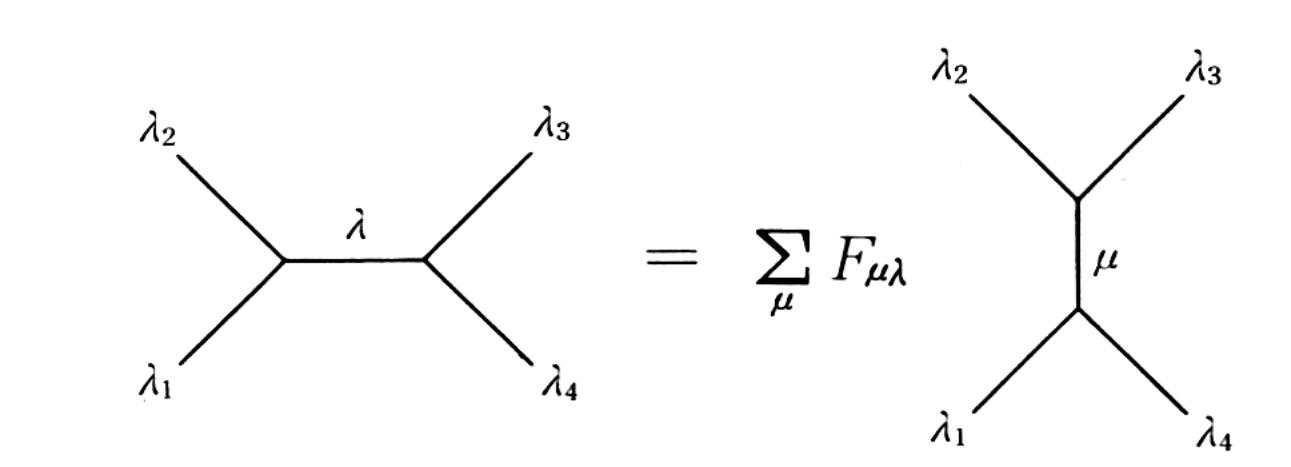
\includegraphics[width=0.70\textwidth]{figures/fig2.2.png}
  \figtitle{2.2}{连接矩阵的图表示（原书 p.56）}
\end{figure}

此前的讨论用到了一点：解可表为式 (2.13) 那样的形状而不出现对数项。这一点也可以从下述事实看出：KZ 方程的解的基，可以表为第 1.6 节所定义的顶点算子的复合。

说明一下：这里讨论的 $n=3$ 的情形，KZ 方程归结为以 $0,1,\infty$ 为正则奇点的一元 Fuchs 型微分方程，连接矩阵可以用一元函数的语言来叙述。$n=3$ 时，KZ 方程 (2.5) 具有如下形状的解：
\begin{equation}
  \Phi(z_1,z_2,z_3)
  =(z_3-z_1)^{\frac{1}{\kappa}(\Omega_{12}+\Omega_{13}+\Omega_{23})}
  G\left(\frac{z_2-z_1}{z_3-z_1}\right), \tag{2.17}
\end{equation}
而 $G$ 满足微分方程
% [原文 p.57]
\begin{equation}
  G'(x)=\frac{1}{\kappa}\left(\frac{\Omega_{12}}{x}+\frac{\Omega_{23}}{x-1}\right)G(x). \tag{2.18}
\end{equation}
这一点可以验证。

在实开区间 $0<x<1$ 上，取微分方程 (2.18) 的基本解系中分别在 $x=0$、$x=1$ 附近表为
\[
\begin{aligned}
  G_0(x)&=x^{\frac{1}{\kappa}\Omega_{12}}H_0(x),\\
  G_1(x)&=(1-x)^{\frac{1}{\kappa}\Omega_{23}}H_1(x),\\
\end{aligned}
\]
（其中 $H_0(x),H_1(x)$ 是单值全纯的）这样的形状的 $G_0(x),G_1(x)$ 来考虑。通过解析延拓可知，存在与 $x$ 无关的矩阵 $F$，使
\begin{equation}
  G_1(x)=G_2(x)F \tag{2.19}
\end{equation}
成立。这个矩阵 $F$ 与由 $\Phi_1=\Phi_2F$ 定义的是同一个。

% [Tutor Note: 原书 p.57 式 (2.19) 作 $G_2$，但 $G_2$ 全书未定义；按上下文（$G_0$ 在 $x=0$ 附近、$G_1$ 在 $x=1$ 附近，解析延拓给出二者的关系）此处应为 $G_0$。正文照录原书。]

此前的讨论是在 $k$ 为正整数、level $k$ 的共形块的空间上进行的；但把参数 $k$ 取为一般值，在 Verma 模不可约的情形下也可以作同样的构造。此外，在上述情形中把 $X=\Omega_{12}$、$Y=\Omega_{23}$ 看作非交换的形式变量，把给出连接的 $F$ 表成 $X,Y$ 的幂级数，所得的对象称为 Drinfel'd associator（结合子）。

如图 2.3 所示，考虑这样的图：它有 $n+1$ 个顶点位于圆周上，每条边都含于圆内，
% [原文 p.58]
圆内每个顶点处都汇聚 3 条边，并且图本身是可缩的。这样的图称为具有 $n+1$ 条外线的树形图（tree）。

% [Tutor Note: 树形图基的关键在于：对每个 $k$，$\sum_{1\le i<j\le k}\Omega_{ij}$ 在该基下同时对角化。因此 (2.20)、(2.21) 中 $u_k$、$v_k$ 的指数可以逐项写出而不出现混合项，这也是后续把所有连接矩阵归结到 $n=3$ 的依据。]

\begin{figure}[htbp]
  \centering
  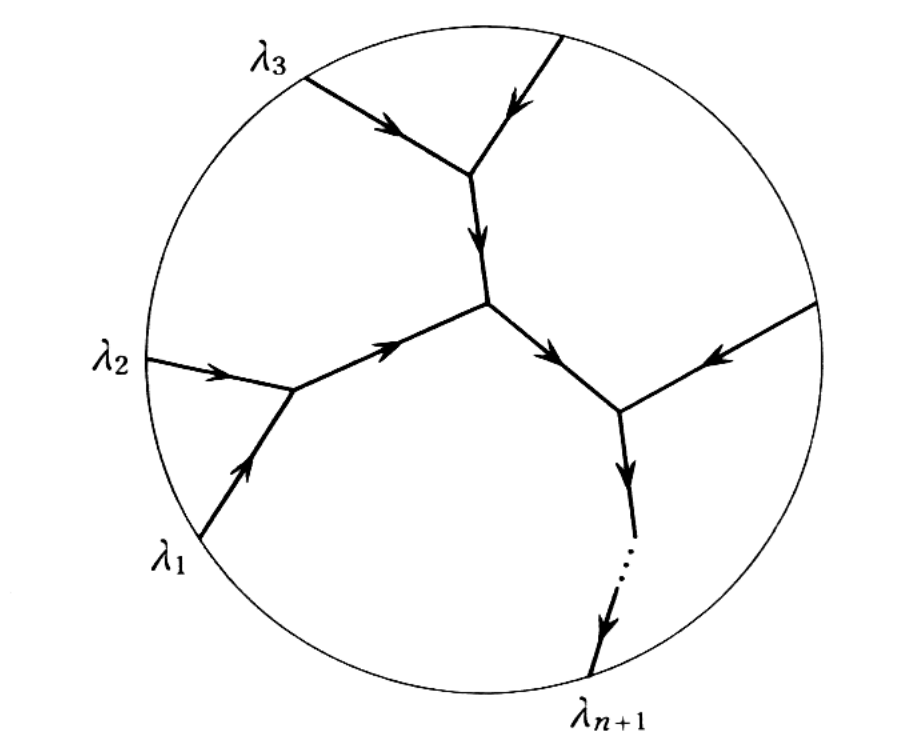
\includegraphics[width=0.50\textwidth]{figures/fig2.3.png}
  \figtitle{2.3}{具有 $n+1$ 条外线的树形图（原书 p.57）}
\end{figure}

对一般的 $n$，自然推广上面说明的 $n=3$ 情形的构造，即可对具有 $n+1$ 条外线的树形图，定义构形空间 $\Conf_n(\C)$ 的部分紧化与 KZ 方程的正规化解。例如，令 $z_1=0$，作坐标变换 $z_{k+1}=u_ku_{k+1}\cdots u_{n-1}$（$k=1,\dots,n-1$），则在 $u_1=\cdots=u_{n-1}=0$ 附近可以考虑如下形状的解：
\begin{equation}
  \Phi_1
  =u_1^{\frac{1}{\kappa}\Omega_{12}}
  u_2^{\frac{1}{\kappa}(\Omega_{12}+\Omega_{13}+\Omega_{23})}
  \cdots
  u_{n-1}^{\frac{1}{\kappa}\sum_{1\le i<j\le n}\Omega_{ij}}
  h_1(u_1,\dots,u_{n-1}), \tag{2.20}
\end{equation}
其中 $h_1(u_1,\dots,u_{n-1})$ 是单值全纯的。此时应注意：在给各边赋予权的树形图所对应的共形块的空间的基上，形式
\[
  \sum_{1\le i<j\le k}\Omega_{ij},\qquad 2\le k\le n
\]
被同时对角化。

图 2.4 是 $n=4$ 的情形，解 (2.20) 对应最上面那类树形图。对于其下一层右方的树，令 $z_1=0$，作坐标变换 $z_2=v_1v_3$、$z_4-z_3=v_2v_3$、$z_4=v_3$，便有由
\begin{equation}
  \Phi_2
  =v_1^{\frac{1}{\kappa}\Omega_{12}}
  v_2^{\frac{1}{\kappa}\Omega_{34}}
  v_3^{\frac{1}{\kappa}\sum_{1\le i<j\le 4}\Omega_{ij}}
  h_2(v_1,v_2,v_3) \tag{2.21}
\end{equation}
表出的解 $\Phi_2$ 与之对应。这里 $h_2(v_1,v_2,v_3)$ 是单值全纯函数。在区域 $z_1<z_2<z_3<z_4$ 上考虑
\begin{equation}
  \lim_{z_2\to z_1}\Phi_i\cdot(z_2-z_1)^{-\frac{1}{\kappa}\Omega_{12}},
  \qquad i=1,2 \tag{2.22}
\end{equation}
即可看出：给出这两个解之间关系的连接矩阵，正是已经考察过的 $n=3$ 情形的连接矩阵。这样，一般地，给出不同树形图所对应解之间关系的连接矩阵，都可以归结为 $n=3$ 的情形。

$n=4$ 时，利用 KZ 联络是平坦联络这一点，可以证明下述命题。
% [原文 p.59]

\begin{figure}[htbp]
  \centering
  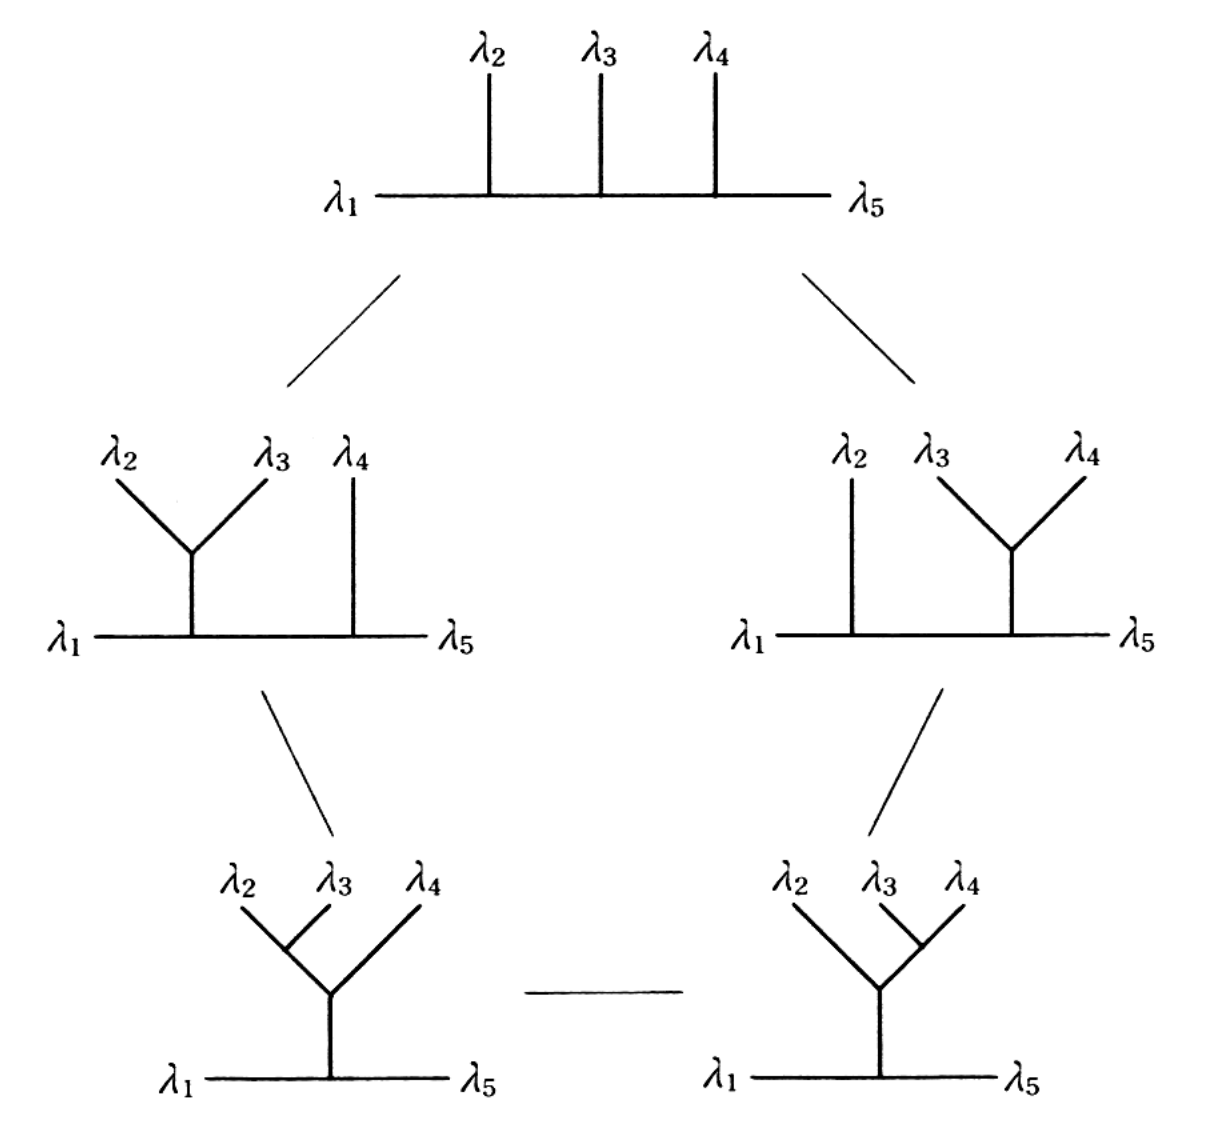
\includegraphics[width=0.55\textwidth]{figures/fig2.4.png}
  \figtitle{2.4}{五边形关系式（原书 p.59）}
\end{figure}

\begin{proposition}{2.2}
  （五边形关系式）如图 2.4 所示，$n=4$ 时的两棵树之间连接它们的路径有两种，而对应于这两条路径的连接矩阵相等。
\end{proposition}

% [Tutor Note: 命题 2.2 就是结合子满足的五边形公理：两种“先合并哪一对”的路径给出同一连接矩阵。把图 2.4 的图换成它们的对偶图即得标准的 pentagon，这也是 Drinfel'd associator 定出辫群表示的原因。]

下面考察作为 KZ 方程的单值而得到的辫群的表示。在实轴上取 $p_1,p_2,\dots,p_n$，使其坐标 $z_1,z_2,\dots,z_n$ 满足 $0<z_1<z_2<\cdots<z_n$，并对这些点配上 $A_1^{(1)}$ 型仿射 Lie 代数 level $k$ 的最高权 $\lambda_1,\dots,\lambda_n$。此外，另取 $p_0,p_{n+1}$，使它们的坐标分别为 $0,\infty$，并对它们配上最高权 $\lambda_0=0$、$\lambda_{n+1}=0$。对于 $\bm{p}=(p_0,p_1,\dots,p_n,p_{n+1})$ 与 $\bm{\lambda}=(\lambda_0,\lambda_1,\dots,\lambda_{n+1}^*)$，共形块的空间 $\cH(\bm{p},\bm{\lambda})$ 如引理 1.13 所示，可以通过多重线性映射的限制嵌入不变张量空间 $\Hom_{\fg}\Bigl(\bigotimes_{j=1}^{n}V_{\lambda_j},\C\Bigr)$；因此以下把它的像与共形块的空间等同，在这里用 $V_{\lambda_1\cdots\lambda_n}$ 来表示。此处，把 $\cH_{\lambda_j}$ 换为对偶模 $\cH_{\lambda_j}^*$
% [原文 p.60]
后再作同样的构造，所得的共形块空间则用最高权 $\lambda_j^*$ 的表记加以区别。

对于辫群 $B_n$ 的生成元 $\sigma_i$，由沿 $\sigma_i$ 所表示的 $\Conf_n(\C)$ 的道路的 KZ 联络的和乐，定出线性映射
\[
  \rho(\sigma_i):V_{\lambda_1\cdots\lambda_i\lambda_{i+1}\cdots\lambda_n}
  \longrightarrow V_{\lambda_1\cdots\lambda_{i+1}\lambda_i\cdots\lambda_n}.
\]
这里 $V_{\lambda_1\cdots\lambda_{i+1}\lambda_i\cdots\lambda_n}$ 表示把点 $p_i,p_{i+1}$ 的位置互换所得的共形块的空间（图 2.5）。如前所述，KZ 联络是平坦联络，故应注意：这个线性映射只由道路的同伦类决定。这样，一般地，对 $\sigma\in B_n$，线性映射
\[
  \rho(\sigma):V_{\lambda_1\cdots\lambda_n}\longrightarrow V_{\lambda_{p(1)}\cdots\lambda_{p(n)}}
\]
同样由 KZ 联络的和乐得到。这里 $p$ 表示辫子 $\sigma$ 所诱导的 $n$ 个文字的置换。进而可知，关于辫子的合成，$\rho$ 满足
\[
  \rho(\sigma\tau)=\rho(\sigma)\rho(\tau),\qquad \sigma,\tau\in B_n.
\]
\begin{figure}[htbp]
  \centering
  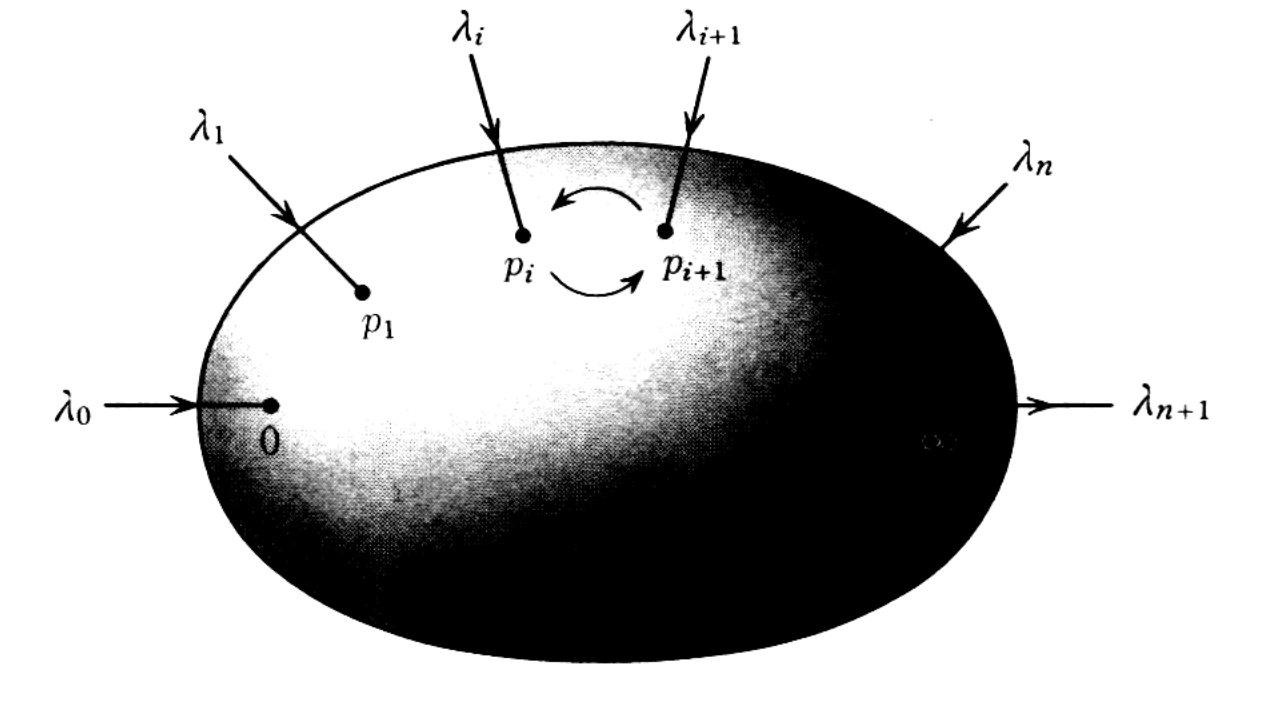
\includegraphics[width=0.82\textwidth]{figures/fig2.5.png}
  \figtitle{2.5}{辫子 $\sigma_i$ 在共形块空间上的作用（原书 p.60）}
\end{figure}

要局部地看辫子的作用，只需注意共形块的特殊基即可。先考虑 $n=3$ 的情形。对于式 (2.13) 所定义的解 $\Phi_1$，辫子 $\sigma_1$ 的作用由 $P_{12}\exp\left(\frac{\pi\sqrt{-1}}{\kappa}\Omega_{12}\right)$ 给出，
% [原文 p.61]
这一点可以看出来。这里 $P_{12}$ 表示交换对应于 $\lambda_1,\lambda_2$ 的张量积分量。在这组基下，应注意 $\Omega_{12}$ 是对角化的。另一方面，对于辫子 $\sigma_2$ 的作用，对式 (2.15) 所定义的解 $\Phi_2$，它由 $P_{23}\exp\left(\frac{\pi\sqrt{-1}}{\kappa}\Omega_{23}\right)$ 给出。此时 $\Omega_{23}$ 对角化。这样，在各自的解的基上可以描述 $\sigma_1,\sigma_2$ 的作用；而辫群的整体作用的描述，则由连接矩阵 $F$ 给出。进一步，与本节对树形图所对应解的连接矩阵的考察相同，对一般的 $n$，辫子 $\sigma_i$ 的作用也归结为 $n=3$ 时的计算，即局部单值的计算与连接矩阵 $F$ 的计算。

% [Tutor Note: $P_{12}$ 是张量积因子置换算子，$\Omega_{12}$ 是 Casimir 作用；二者交换，故指数量 $P_{12}\exp(\cdots\Omega_{12})$ 可按 $\Omega_{12}$ 的特征分解逐项计算。这里的 $\sqrt{-1}$ 与 $\kappa$ 的配合决定了固有值是否为实数。]

下面考虑 Lie 代数 $\fg$ 为 $\fsl_2(\C)$、表示 $V_{\lambda_1},\dots,V_{\lambda_n}$ 均为二维不可约表示的情形。此时，按上面说明的方法考察 $(z_{i+1}-z_i)^{\frac{1}{\kappa}\Omega_{i,i+1}}$ 这一部分的多值性，即可计算单值矩阵 $\rho(\sigma_i)$ 的特征值。令 $q^{\frac{1}{2}}=\exp(\pi\sqrt{-1}/\kappa)$、$\eta=\exp(\pi\sqrt{-1}/2\kappa)$，则可知 $g_i=\eta\rho(\sigma_i)$ 满足关系式
\begin{equation}
  (g_i-q^{\frac{1}{2}})(g_i+q^{-\frac{1}{2}})=0. \tag{2.23}
\end{equation}
把生成元 $\sigma_i$ 对应到上述 $g_i$ 所得的辫群的表示，记作
\[
  \tilde\rho:B_n\longrightarrow\End(V_{\lambda_1\cdots\lambda_n}).
\]
一般地，对于非零的复参数 $q$，在 $\C$ 上由 $1,T_i$（$1\le i\le n-1$）生成、且满足关系式
\[
\begin{aligned}
  &T_iT_{i+1}T_i=T_{i+1}T_iT_{i+1}, && i=1,\cdots,n-2,\\
  &T_iT_j=T_jT_i, && |i-j|>1,\\
  &(T_i-q^{\frac{1}{2}})(T_i+q^{-\frac{1}{2}})=0
\end{aligned}
\]
的代数，称为 Iwahori--Hecke 代数（岩堀--Hecke 代数），记作 $H_n(q)$。

% [Tutor Note: 引入 $\eta$ 是为把 $\rho(\sigma_i)$ 的特征值写成 $q$ 的幂次的对称形状；由 (2.23) 直接看出 $\tilde\rho(\sigma_i)=g_i$ 已满足 Iwahori--Hecke 代数的二次关系 $(T_i-q^{1/2})(T_i+q^{-1/2})=0$。]

% [原文 p.62]
把上面的考察归纳起来，便证明了下述定理。

\begin{theorem}{2.3}
  由 Lie 代数 $\fsl_2(\C)$ 及其二维不可约表示所定义的 KZ 方程，其单值所给出的辫群的表示 $\tilde\rho:B_n\to\End(V_{\lambda_1\cdots\lambda_n})$，给出 Iwahori--Hecke 代数 $H_n(q)$ 的表示。
\end{theorem}

\begin{figure}[htbp]
  \centering
  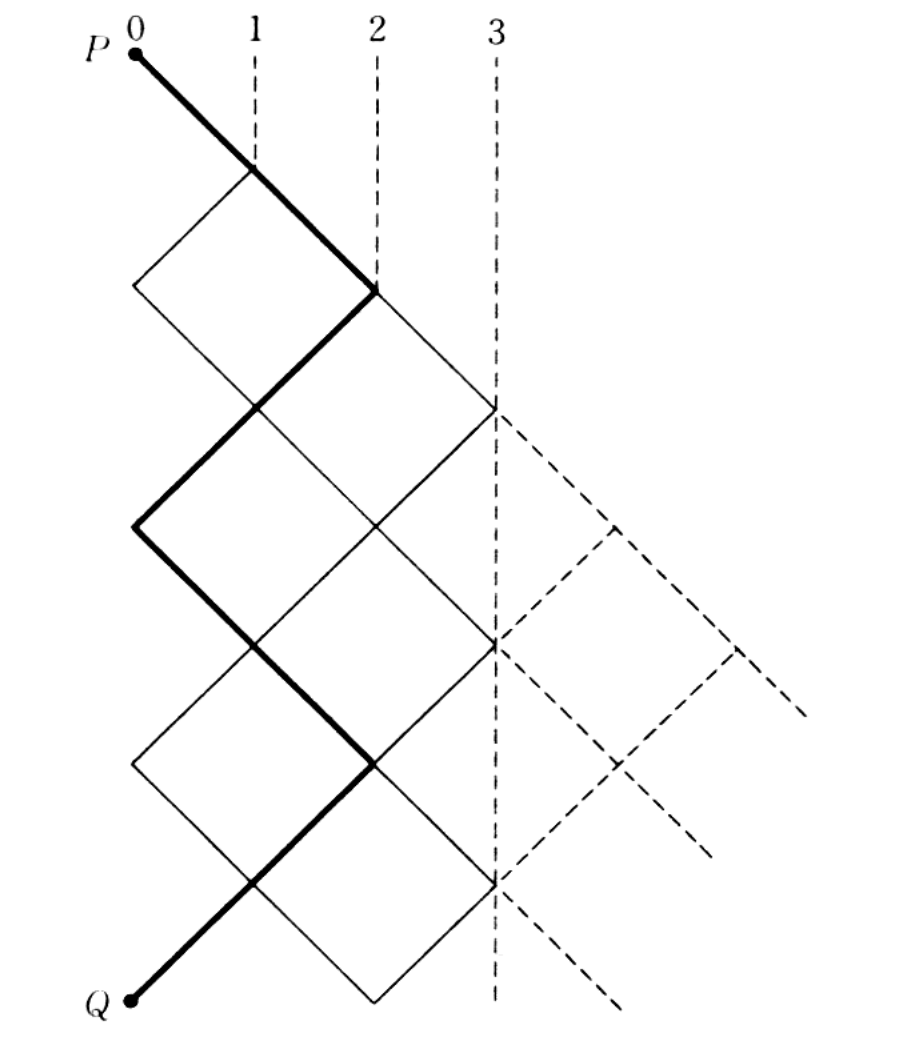
\includegraphics[width=0.42\textwidth]{figures/fig2.6.png}
  \figtitle{2.6}{$k=3$、$n=7$ 的情形；表示空间的基与实线上连接 $P$ 与 $Q$ 的最短路径相对应。（原书 p.62）}
\end{figure}

% [Tutor Note: 定理 2.3 的证明在此只用“归纳上面的考察”一句带过。实际上需要验证 $\tilde\rho$ 满足 (2.1)、(2.2) 与 (2.23) 三组关系；其中辫关系由 KZ 联络在 $\Conf_n(\C)$ 上的平坦性保证（同伦不变），二次关系由 (2.23) 直接给出。]

已知这里出现的辫群的表示是不可约酉表示（参见文献 [44]）。表示空间的基与图 2.6 所示的路径相对应。表示空间的基之所以受到由 level $k$ 确定的限制，其依据在于命题 1.14 所得的、共形块空间所满足的代数关系式。具体说来，基由命题 1.15 的融合规则描述。如本节所述，辫子作用的计算归结为 $n=3$ 的情形。此时共形块的空间至多为二维，KZ 方程化为 Gauss 超几何微分方程。因此，可以利用超几何函数的连接具体地描述辫群的作用。又，把定理 2.3 推广到 $\fg=\fsl_m(\C)$、$V_{\lambda_1},\dots,V_{\lambda_n}$ 为 $m$ 维自然表示的情形，也是可以做到的。

% 块尾跨页句：p.62 末句「また，定理 2.3 を，g=sl_m(C) で，…」续至 p.63 页首「張することもできる．」，已在此译完；ch02b 请从 p.63「この場合は，κ=k+m，…」起接译。
% CHUNK ch02a DONE
